\chapter{Young Entrepreneur Interviews SHAQ}

This chapter follows the School of Hard Knocks interview with Dr. Shaquille O'Neal as evidence for a practical theory of scale. The mathematics here is deliberately modest: the transcript is not a physics lecture, and there are no validated board frames. But the interview contains a real quantitative spine. It asks how one person moves from athletic income to durable ownership, how a single owner can be connected to many businesses, and why the mechanics of keeping money differ from the mechanics of making it.

\section{Fame Is Not the Mechanism}

The opening is a cold start. The interviewer asks who is present, and the answer is direct: Dr. Shaquille O'Neal. Then the categories come quickly. He names many industries, and later the full interview gives examples: DJing, law enforcement, food and beverages, and pizza. The point is not to make a list of celebrity ventures. The point is to put pressure on a question: what is the mechanism that lets a person with one body and one schedule touch many enterprises?

The teaser gives the number that sets up the whole problem. The interviewer says that Shaq owned 155 Five Guys locations at one point, and Shaq answers that he sold them. We record that as an interview claim, not as an audited corporate inventory:

\begin{equation}
N_{\mathrm{Five\ Guys}} = 155.
\end{equation}

A number like \(155\) is already larger than personal supervision. It is not a question of working harder in the ordinary sense. If one owner must personally appear at each location, then the model breaks before it begins. So the interview immediately turns celebrity into an operating constraint.

\section{Delegation And The 155-Place Constraint}

The interviewer asks for the secret to scaling in the franchise model, or in business generally. Shaq answers with one word: delegation. Then he gives the physical reason: he cannot be in 155 places at once, but he knows somebody who can.

Let \(N\) denote the number of locations and let \(C_{\mathrm{one}}\) denote the direct operating capacity of one person. The problem is not subtle:

\begin{equation}
N_{\mathrm{locations}} > C_{\mathrm{one}}.
\end{equation}

When \(N=155\), the owner cannot be the whole operating system. The only way to make the inequality workable is to introduce other people whose judgment and labor extend coverage. If there are \(m\) delegated operators, and operator \(i\) can responsibly cover capacity \(c_i\), then the clean reconstructed condition is

\begin{equation}
N_{\mathrm{covered}} \leq \sum_{i=1}^{m} c_i.
\end{equation}

This is not a formula Shaq writes on a board. It is the minimal mathematical reconstruction of his sentence. The spoken claim is simpler: scale is not being everywhere; scale is knowing who can be somewhere for you.

\begin{figure}
\centering
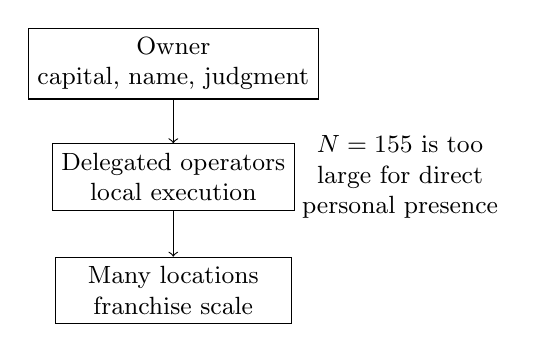
\begin{tikzpicture}[scale=0.9, every node/.style={font=\small}]
\node[draw, align=center, minimum width=3.0cm, minimum height=0.8cm] (owner) at (0,0) {Owner\\capital, name, judgment};
\node[draw, align=center, minimum width=3.0cm, minimum height=0.8cm] (ops) at (0,-1.6) {Delegated operators\\local execution};
\node[draw, align=center, minimum width=3.0cm, minimum height=0.8cm] (sites) at (0,-3.2) {Many locations\\franchise scale};
\draw[->] (owner) -- (ops);
\draw[->] (ops) -- (sites);
\node[align=center] at (3.2,-1.6) {\(N=155\) is too\\large for direct\\personal presence};
\end{tikzpicture}
\caption{A transcript-derived reconstruction of the delegation mechanism: one owner cannot personally cover many locations, so operating capacity must pass through trusted people.}
\end{figure}

\subsection{Question \& Answer}

\paragraph{Question.}
How can one owner scale beyond personal attention?

\paragraph{Answer.}
By separating ownership from direct presence. In the interview, the obstruction is physical: one person cannot be in 155 places at once. The resolution is organizational: find and trust capable operators. The owner still controls the strategy, reputation, capital, and choice of people, but execution is distributed.

That answer also explains why Shaq connects business to championships later in the interview. Teams are not decoration. They are the operating machinery.

\section{Stealing Models And Building A Self}

After the Atlanta reset, the host frames Shaq as an NBA legend, a business mogul, and a figure claimed to have a net worth above 500 million dollars. The interview then returns to identity: who are you, what industries did you pursue, what were you doing before business? Shaq jokes that before becoming a business mogul he was killing the interviewer's favorite NBA player.

The serious turn comes when the interviewer asks about the biggest driving factor in his success. Shaq says, ``I was a thief,'' and then explains the term. If somebody is doing better and you aspire to be like them, steal what they are doing. He names Michael Jordan, Magic Johnson, Kareem Abdul-Jabbar, and Muhammad Ali, and says he put those influences inside his brain to create Shaquille O'Neal.

We can write the mechanism without pretending it is a literal equation of identity. Let \(M_j\) be a model and \(s_j\) be a skill, discipline, or pattern extracted from that model. Then the practical update rule is

\begin{equation}
\mathrm{Self}_{t+1}
=
\mathrm{Self}_{t}
+
\sum_{j=1}^{k} w_j s_j
+
r.
\end{equation}

Here \(w_j\) is the weight given to model \(j\), and \(r\) is the personal remainder: taste, temperament, timing, and what Shaq later calls adding your own style. The formula is only a reconstruction. The transcript's language is sharper than the notation: watch, steal, combine, become.

\section{Keeping Money After Making It}

The interviewer then introduces a different tension. Making money and keeping money are not the same operation. He cites a claim that one in three NFL players go broke within three to five years, and he asks how to preserve large earnings when a lot of money is suddenly dumped on a person.

We should keep the claim as spoken evidence, not as external proof:

\begin{equation}
\mathrm{claimed\ broke\ rate} = \frac{1}{3}
\quad \mathrm{within}\quad 3\text{--}5\ \mathrm{years}.
\end{equation}

Shaq's answer is deliberately short: for people who are not financially literate, learn the word annuity. He does not give a classroom derivation, and the final chapter should not pretend that he did. But we can say what the word is doing in the conversation. It points away from treating wealth as a pile to spend and toward treating wealth as a stream to govern.

A cautious reconstruction is

\begin{equation}
W_0 \longmapsto (P_1,P_2,\ldots,P_T),
\end{equation}

where \(W_0\) is an initial stock of wealth and \(P_t\) are scheduled payments over time. That is enough. The important interview move is conceptual: financial literacy begins when a lump sum is no longer mistaken for a permanent condition.

\subsection{Question \& Answer}

\paragraph{Question.}
Why is making money easier than keeping money?

\paragraph{Answer.}
Because making money can be a single event, while keeping money is a repeated discipline. The transcript gives two sides of that discipline. First, Shaq names annuity as a preservation concept. Later, he describes his early mistake: the first time he received a million dollars, he spent it in about 30 minutes on cars, jewelry or similar items, and suits, while not yet knowing what FICO was. The mechanism is the difference between receiving wealth and having a system for it.

\section{Starting, Franchising, And The Failure Rate}

A promotional interlude interrupts the interview. It names the School of Mentorship and several business figures, including Steven Klubeck, James Keyes, and Cody Sperber. That material is part of the show's context and should not be folded into Shaq's testimony. Its role in the chapter is mainly to reinforce a recurring premise: access to experienced people is treated as economically valuable.

When the interview resumes, the interviewer asks whether someone today should start a business or franchise a business. Shaq answers: both. The distinction is practical. Start a business if one is inspired by something, wants to do it, thinks it will work, and believes it will work. Franchise, or copy a working model, when something is already working and the local situation makes sense.

The host then gives another numerical claim: eight out of ten companies go out of business in five years. Again, this should be marked as the interviewer's claim:

\begin{equation}
\mathrm{claimed\ failure\ rate} = \frac{8}{10},
\qquad
\mathrm{implied\ survival\ rate} = \frac{2}{10}.
\end{equation}

Asked for the most common mistake business owners make, Shaq says they think they know it all. The correction is to hire people smarter than oneself. This returns us to the delegation equation, but now with a sharper condition. It is not enough to add people. The added people must increase the system's intelligence.

\section{Negotiation Arithmetic And Operating Discipline}

The interview then becomes numerical in a more precise way. Asked for negotiation advice, Shaq gives two rules: do not talk first, and start high. His example is compact enough to preserve almost as arithmetic.

Suppose the other side's budget is

\begin{equation}
B = \$200\mathrm{M}.
\end{equation}

If the first ask is too low, say

\begin{equation}
a_0 = \$50\mathrm{M},
\end{equation}

then the value left outside the opening ask is

\begin{align}
L
&= B-a_0 \\
&= \$200\mathrm{M}-\$50\mathrm{M} \\
&= \$150\mathrm{M}.
\end{align}

This is the cleanest worked example in the interview. The transcript also gives a higher-anchor path:

\begin{equation}
\$200\mathrm{M}
\rightarrow
\$110\mathrm{M}
\rightarrow
\$140\mathrm{M}
\rightarrow
\$125\mathrm{M}.
\end{equation}

The exact bargaining logic is conversational, but the lesson is precise. A low anchor does not merely sound modest. If the other side has a larger budget, the low anchor can destroy the negotiator's own upside before the bargaining has properly begun.

The same section also gives a mentor's savings rule:

\begin{equation}
S = 0.75I,
\qquad
F = 0.25I,
\qquad
S+F=I.
\end{equation}

Here \(I\) is income, \(S\) is the saved portion, and \(F\) is the portion used for enjoyment. The rule is not presented as a universal financial theorem. It is a discipline Shaq says he received as advice: save 75 and have fun with 25.

\section{Risk, Teams, And What Gets Missed}

The interview returns to 155 Five Guys and delegation, now with a sports explanation. Shaq says he learned the importance of bringing people in by winning championships. Having great teammates helps one win championships, and the same logic carries into business.

Then the conversation shifts from scale to risk. Asked about the biggest risk he ever took in business, Shaq answers by naming an opportunity he did not take. He says Howard Schultz wanted to open Starbucks in the hood, and Shaq misunderstood the opportunity because he did not yet understand re-gentrification and re-beautification of certain areas. He says he did not pull the trigger, and that Magic Johnson later opened many Starbucks.

The lesson is not simply that every opportunity should be taken. It is that the language of an opportunity can hide its actual economic mechanism. Shaq heard one meaning of ``the hood.'' The business case apparently depended on another meaning: changing neighborhoods, changing consumer demand, and the value of being early.

Later, he gives a cleaner investment rule, attributed in spirit to Jeff Bezos: invest in things that will change people's lives. He also says that when he invests in a person, he wants to believe in what they believe in. So the investment criterion is not only asset class or industry. It is a fit between belief, utility, and person.

\section{Luck, Belief, And The Beginner Blueprint}

Near the end, the interviewer asks how Shaq found the self-belief to make hundreds of millions of dollars. Shaq complicates the premise. He says he had an athletic advantage: he was given a lot of money to play sports, then he leveraged that money and did certain things. He says he can kind of answer the question, but not completely, because for him it was luck.

That admission matters. It prevents the chapter from turning the interview into a simple recipe. There are mechanisms: delegation, imitation, annuity, savings discipline, high anchoring, smarter hires. But there is also path dependence. Shaq begins with unusual athletic income. He then has to learn how not to waste it, how to place it, and how to let other people operate around it.

The final advice returns to the motif of model theft. If you have a plan, write it down and figure it out. If somebody else is already doing what you want to do, watch them, steal what they are doing, and add your own razzmatazz. Expect ups and downs, and keep believing long enough for the process to work.

This closes the loop opened at the beginning. The athlete becomes the owner not by replacing all ordinary mechanisms, but by passing through them: copying, delegating, preserving, negotiating, missing, learning, and trying again.

\section{Summary}

The transcript gives a compact theory of business scale through Shaq's interview answers. The first law is the 155-place constraint: if \(N\) is larger than one person's direct capacity, delegation is not optional. The second law is preservation: a lump sum is not durable wealth unless it is governed by financial literacy, savings discipline, and structures such as annuities. The third law is leverage through people: imitate useful models, hire smarter operators, negotiate from strength, and invest where belief and usefulness meet.

No validated mathematical screenshots survive for this lecture, so the equations and diagrams in this chapter are reconstructions from the transcript rather than blackboard readings. The evidence remains the spoken sequence: fame opens the door, but the repeated mechanisms are people, discipline, and judgment.